\documentclass[12pt]{article}
\input{preamble}

\pagestyle{fancy}
\fancyhf{}



%Husk at rette modul og dato!

\cfoot{Side \thepage \hspace{1pt} af \pageref{LastPage}}

\begin{document}
\begin{titlepage}
\begin{center}
    \Large
    \textbf{RSA-kryptosystemet}
        
    \vspace{0.4cm}
    \large
     Nørre Gymnasium\\
     SRO 2.e
        

\end{center}
\end{titlepage}

%Udfyld afsnit herunder og lav til egen Latex-fil

%Kopier følgende til overskrift:

%\begin{center}
%\Huge
%Aflevering 1
%\end{center}
%\section*{Opgave 1}
%\stepcounter{section}



\section{Kort om kryptologi}


Vi vil begynde med at skabe os en forståelse for, hvad kryptologi det er. Dette vil vi gøre gennem tænkte eksempler, hvor vi løbende introducerer terminologi. Vi vil starte med at introducere et simpelt \textit{kryptosystem}, der beskriver idéen bag kryptologi, men har store sikkerhedsbrister. Dette er det såkaldte \textit{Cæsar-chiffer}, som efter sigende skulle være udtænkt af Julius Cæsar. Et eksempel på et mere berømt kryptosystem er Enigma, der under anden verdenskrig blev brugt af Nazityskland til at sende hemmelige beskeder indbyrdes. 

\subsubsection*{Terminologi}
Begrebet kryptologi dækker overordnet over to begreber: Det at skabe kryptosystemer, som Cæsar-chifferet eller Enigma, som vi kalder for \textit{Kryptografi}, og det at bryde eller knække kryptosystemer, som vi kalder for \textit{Kryptoanalyse}. Et \textit{chiffer} er en algoritme, der kan bruges til \textit{kryptering} og \textit{dekryptering}. Kryptering består i at gøre en tekst eller lignende ulæseligt for uvedkommende og dekryptering er den omvendte proces. Vi kalder den ukrypterede tekst for \textit{klarteksten}, og den krypterede tekst for \textit{chifferteksten}. Klarteksten og chifferteksten består begge af \textit{bogstaver} fra et \textit{alfabet}. Bemærk, at et alfabet ikke nødvendigvis behøver at bestå af A-Å, men kan også består af tal, figurer eller alt muligt andet. Klartekst-alfabetet og chiffertekst-alfabetet behøver heller ikke at være ens. Vi betegner mængden af alle klartekster med $\mathscr{P}$ og mængden af alle chiffertekster med $\mathscr{C}$. Til slut har vi en \textit{krypteringsfunktion} $e:\mathscr{P} \to \mathscr{C}$, der krypterer klartekster til chiffertekster, og en dekrypteringsfunktion $d:\mathscr{C} \to \mathscr{P}$, der dekrypterer chiffertekster til klartekster. Vi ønsker selvfølgelig, at for alle klartekster $m\in \mathscr{P}$, at der gælder, at 
\begin{align*}
d(e(m)) = m,
\end{align*}
altså at kryptering af en besked og en efterfølgende dekryptering giver os den oprindelige besked tilbage. Princippet bag et kryptosystem kan ses af diagrammet i Fig. \ref{fig:krypto},
\begin{figure}[H]
\centering
\begin{tikzpicture}
\node at (0,0) (1) {$\mathscr{P}$};
\node at (2,0) (2) {$\mathscr{C}$};
\node at (4,0) (3) {$\mathscr{P}$};
\node at (1,0.3) {$e$};
\node at (3,0.3) {$d$};
\draw[->] (1) to (2);
\draw[->] (2) to (3);
\end{tikzpicture}
\caption{Kryptosystem}
\label{fig:krypto}
\end{figure}

\subsection*{Cæsar-chiffer}
Om Cæsar rent faktisk selv opfandt Cæsar-chifferet er svært at afgøre, men det er forståeligt, hvorfor de i Romerriget kan have haft brug for kryptografi af forskellig art. Hvis senatet og kejseren i Rom blev enige om at ændre krigsstrategi i udkanten af riget, så var en besked lang tid undervejs, og romerne var selvfølgelig ikke interesserede i, at beskeden skulle falde i deres modstanderes hænder. At gøre denne besked ulæselig for uvedkommende vil derfor have været et kærkomment redskab. 

Cæsar-chifferet er ret simpelt. Alfabetet er vores sædvanlige alfabet $\{\textnormal{A,B},\hdots,\textnormal{Å}\}$,
og både $\mathscr{P}$ og $\mathscr{C}$ består af alle mulige bogstavkombinationer. Krypteringsfunktionen $e_k:\mathscr{P} \to \mathscr{C}$ består i at forskyde alle bogstaver $k$ pladser til højre i alfabetet, og vi kalder $k$ for \textit{krypteringsnøglen}. I tilfældet at $k = 2$, så vil A blive til C, B til D osv. Dekrypteringsfunktionen $d_k$ forskyder tilsvarende alle bogstaver $k$ pladser til venstre i alfabetet. Fig. \ref{fig:caesar} beskriver kryptering for dette kryptosystem. Dekryptering foregår tilsvarende ved at gå mod pilenes retning i figuren. 
\begin{figure}[H]
\centering
\resizebox{\textwidth}{!}{
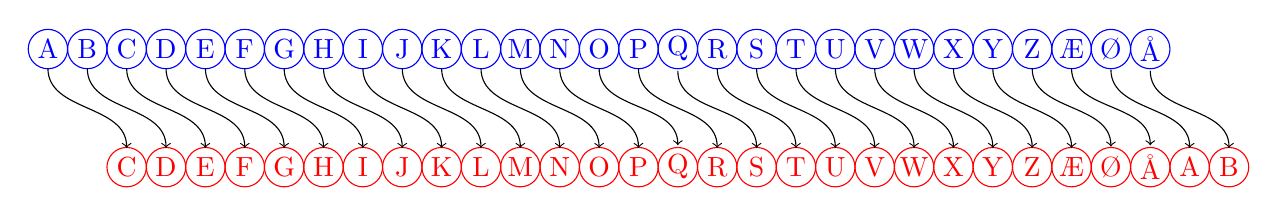
\begin{tikzpicture}
\foreach \i in {1,...,29}
{
     \draw[color=blue] (\i * 0.5 ,0) circle (0.25 cm);
}
\node[color = blue] at (0.5,0) (1) {A};
\node[color = blue] at (1,0) (2) {B};
\node[color = blue] at (1.5,0) (3) {C};
\node[color = blue] at (2,0) (4) {D};
\node[color = blue] at (2.5,0) (5) {E};
\node[color = blue] at (3,0) (6) {F};
\node[color = blue] at (3.5,0) (7) {G};
\node[color = blue] at (4,0) (8) {H};
\node[color = blue] at (4.5,0) (9) {I};
\node[color = blue] at (5,0) (10) {J};
\node[color = blue] at (5.5,0) (11) {K};
\node[color = blue] at (6,0) (12) {L};
\node[color = blue] at (6.5,0) (13) {M};
\node[color = blue] at (7,0) (14) {N};
\node[color = blue] at (7.5,0) (15) {O};
\node[color = blue] at (8,0) (16) {P};
\node[color = blue] at (8.5,0) (17) {Q};
\node[color = blue] at (9.0,0) (18) {R};
\node[color = blue] at (9.5,0) (19) {S};
\node[color = blue] at (10,0) (20) {T};
\node[color = blue] at (10.5,0) (21) {U};
\node[color = blue] at (11.0,0) (22) {V};
\node[color = blue] at (11.5,0) (23) {W};
\node[color = blue] at (12.0,0) (24) {X};
\node[color = blue] at (12.5,0) (25) {Y};
\node[color = blue] at (13,0) (26) {Z};
\node[color = blue] at (13.5,0) (27) {Æ};
\node[color = blue] at (14,0) (28) {Ø};
\node[color = blue] at (14.5,0) (29) {Å};

\foreach \i in {1,...,29}
{
     \draw[color=red] (\i * 0.5+1 ,-1.5) circle (0.25 cm);
}
\node[color = red] at (15,-1.5) (30) {A};
\node[color = red] at (15.5,-1.5) (31) {B};
\node[color = red] at (1.5,-1.5) (32) {C};
\node[color = red] at (2,-1.5) (33) {D};
\node[color = red] at (2.5,-1.5) (34) {E};
\node[color = red] at (3,-1.5) (35) {F};
\node[color = red] at (3.5,-1.5) (36) {G};
\node[color = red] at (4,-1.5) (37) {H};
\node[color = red] at (4.5,-1.5) (38) {I};
\node[color = red] at (5,-1.5) (39) {J};
\node[color = red] at (5.5,-1.5) (40) {K};
\node[color = red] at (6,-1.5) (41) {L};
\node[color = red] at (6.5,-1.5) (42) {M};
\node[color = red] at (7,-1.5) (43) {N};
\node[color = red] at (7.5,-1.5) (44) {O};
\node[color = red] at (8,-1.5) (45) {P};
\node[color = red] at (8.5,-1.5) (46) {Q};
\node[color = red] at (9.0,-1.5) (47) {R};
\node[color = red] at (9.5,-1.5) (48) {S};
\node[color = red] at (10,-1.5) (49) {T};
\node[color = red] at (10.5,-1.5) (50) {U};
\node[color = red] at (11.0,-1.5) (51) {V};
\node[color = red] at (11.5,-1.5) (52) {W};
\node[color = red] at (12.0,-1.5) (53) {X};
\node[color = red] at (12.5,-1.5) (54) {Y};
\node[color = red] at (13,-1.5) (55) {Z};
\node[color = red] at (13.5,-1.5) (56) {Æ};
\node[color = red] at (14,-1.5) (57) {Ø};
\node[color = red] at (14.5,-1.5) (58) {Å};

\draw[->] (1) to [out = -90,in = 90] (32);
\draw[->] (2) to [out = -90,in = 90] (33);
\draw[->] (3) to [out = -90,in = 90] (34);
\draw[->] (4) to [out = -90,in = 90] (35);
\draw[->] (5) to [out = -90,in = 90] (36);
\draw[->] (6) to [out = -90,in = 90] (37);
\draw[->] (7) to [out = -90,in = 90] (38);
\draw[->] (8) to [out = -90,in = 90] (39);

\draw[->] (9) to [out = -90,in = 90] (40);
\draw[->] (10) to [out = -90,in = 90] (41);
\draw[->] (11) to [out = -90,in = 90] (42);
\draw[->] (12) to [out = -90,in = 90] (43);

\draw[->] (13) to [out = -90,in = 90] (44);
\draw[->] (14) to [out = -90,in = 90] (45);
\draw[->] (15) to [out = -90,in = 90] (46);
\draw[->] (16) to [out = -90,in = 90] (47);

\draw[->] (17) to [out = -90,in = 90] (48);
\draw[->] (18) to [out = -90,in = 90] (49);
\draw[->] (19) to [out = -90,in = 90] (50);
\draw[->] (20) to [out = -90,in = 90] (51);

\draw[->] (21) to [out = -90,in = 90] (52);
\draw[->] (22) to [out = -90,in = 90] (53);
\draw[->] (23) to [out = -90,in = 90] (54);
\draw[->] (24) to [out = -90,in = 90] (55);

\draw[->] (25) to [out = -90,in = 90] (56);
\draw[->] (26) to [out = -90,in = 90] (57);

\draw[->] (27) to [out = -90,in = 90] (58);
\draw[->] (28) to [out = -90,in = 90] (30);

\draw[->] (29) to [out = -90,in = 90] (31);

\end{tikzpicture}
}
\caption{kryptering med Cæsar-chiffer hvor $k = 2$}
\label{fig:caesar}
\end{figure}
\begin{exa}
Vi modtager chifferteksten $c=$CPFGP G GNUMGT OCV, og vi ved, at den er krypteret med krypteringsfunktionen $e_2$. Derfor har vi, at 
\[
\textnormal{CPFGP G GNUMGT OCV} = e_2(m),
\]
hvor $m$ er klarteksten. For at finde $m$ bestemmer vi
\[
m = d_2(\textnormal{CPFGP G GNUMGT OCV}).
\]
Dette gøres ved at gå baglens i tabellen i Fig \ref{fig:caesar}, og vi får, at klarteksten er
\begin{align*}
m = \textnormal{ANDEN E ELSKER MAT}.
\end{align*}
\end{exa}
Med dette kryptosystem følger nogle ret store problemer. Hvis chifferteksten $c$ opsnappes af en tredjepart og tredjeparten ved, at beskeden er krypteret med et Cæsar-chiffer, så kan tredjeparten blot prøve alle 29 nøgler for at dekryptere. Dette kan højst tage 29 gange så lang tid som at dekryptere en besked, hvis man ikke kender nøglen, som hvis man kender den, hvilket er alt for kort tid. 

Alternativt kunne man parre bogstaverne på andre måder. Dette ville øge sikkerheden mod et angreb, der består i at afprøve alle nøgler, da man kan parre bogstaverne på 
\[
29! = 8841761993739701954543616000000
\]
måder. Men så kan man udnytte strukturen i en gennemsnitlig tekst. På dansk er det hyppigst brugte bogstav E, der optræder som omtrent $15\%$ af alle bogstaver. Derfor vil det hyppigste bogstav i en chiffertekst formentlig tilsvare E i klarteksten. Denne analyse kan så gennemgåes med det næsthyppigste bogstav, tredjehyppigste osv. indtil chifferteksten kan dechifreres til klarteksten. 

Et kryptosystem som Cæsar-chifferet kaldes for et symmetrisk kryptosystem, da begge parter skal blive enige om en krypteringsnøgle $k$. 

\subsection*{Public-key-kryptosystemer}
RSA-kryptosystemet er et såkaldt public-key-kryptosystem (eller asymmetrisk kryptosystem). Dette betyder, at krypteringsnøglen, der skal bruges til at kryptere klarteksten til chifferteksten er offentligt tilgængelig i den forstand at vi ikke gør noget for at skjule den for tredjeparter. Vi vil gennemgå princippet bag public-key-kryptosystemer uden at komme ind på, hvad RSA gør mere specifikt.

Vi betragter en situation, hvor en person Alice ønsker at sende en krypteret besked til en anden person Bob. Et public-key-system består af følgende skridt:
\begin{enumerate}[label=\roman*)]
\item Bob bestemmer to nøgler: en offentlig nøgle $k_o$ og en privat nøgle $k_p$. Den offentlige nøgle $k_o$ deler han med Alice.
\item Alice bruger nøglen $k_o$ til at kryptere klarteksten $m$ med krypteringsfunktionen $e_k.$ Hun bestemmer altså chifferteksten
\[
c = e_{k_o}(m),
\]
og sender $c$ til Bob. 
\item Bob bruger sin private nøgle $k_p$ sammen med den offentlige nøgle $k_o$ til at bestemme dekrypteringsnøglen $k$. Han dekrypterer nu chifferteksten $c$:
\[
m = d_k(c),
\]
og Bob har modtaget Alices besked. 
\end{enumerate}

\begin{figure}[H]
\centering

{\fontfamily{lmss}\selectfont
\resizebox{\textwidth}{!}{
\begin{tikzpicture}
\node at (0,0) {\includegraphics[scale=0.5]{billeder/alice2.png}};
\node at (5,0) {\includegraphics[scale=0.5]{billeder/bob2.png}};
\node at (0,1.5) {\large Alice};
\node at (5,1.5) {\large Bob};
\node[text width=3cm] at (8,-2.5) {\scriptsize Bob bestemmer  privat nøgle $k_p$ og offentlig nøgle $k_o$ og sender $k_o$ til Alice};
\filldraw[color=blue!25,thick] (4.5,-2) circle (0.3cm);
\filldraw[color=blue!25,thick] (5.5,-2) circle (0.3cm);
\node[color = white, minimum size = 0.3cm] at (4.5,-2) (1) {$k_o$};
\node[color = white] at (5.5,-2) {$k_p$};

\draw[->] (1) to [out = -90,in = 0] (1,-3.5);
\node at (-1,-3.5) (2) {$m=$Hej Bob};
\node at (-1,-5) (3) {$c=\% +0! Ak $};
\draw[->] (2) to (3);
\node at (-0,-4.25) {$e_{k_0}(m)$};
\node[text width = 3cm] at (-4,-4) {\scriptsize Alice bruger den offentlige nøgle $k_o$ til at kryptere klartekst $m$ og sender chiffertekst $c$ til Bob};
\draw[->] (3) to [out = -90, in = 180] (3.5,-6.5);

\node at (5,-6.5) (4) {$\% +0! Ak =c$}; 
\node at (5,-8) (5) {Hej Bob$=m$};
\draw[->] (4) to (5);
\node at (4,-7.25) {$d_{(k_0,k_p)}(c)$};
\node[text width = 3cm] at (8,-7) {\scriptsize Bob bruger sin private nøgle $k_p$ samt den offentlige nøgle $k_o$ til at dekryptere chifferteksten $c$ til klarteksten $m$.};
\end{tikzpicture}
}
}
\caption{Princip i public-key-kryptosystem}
\label{fig:publickey}
\end{figure}

Et godt public-key-kryptosystem skal opfylde, at det er let at beregne $c=e_{k_o}(m)$, men meget svært at beregne $m$ hvis man kun kender $c$ og $k_o$. Det skal desuden være let at beregne $d_{k_o,k_p}(c) = m$, når man kender både den private og offentlige nøgle. RSA-kryptosystemet udnytter, at det er let at gange store primtal sammen, men svært at bestemme hvilke primtalsfaktorer store tal har. 
\subsection*{Opgaver}
\begin{enumerate}[label=\roman*)]
\item Brug krypteringsfunktionen $e_2$ til at kryptere klarteksten 
\[m = \textnormal{HEJ VERDEN}\]
\item Brug dekrypteringsfunktionen til at dekryptere chifferteksten
\[
c = \textnormal{EÅUCTEJKHHCT}
\]
\item Vi har opsnappet chifferteksten 
\[
c = \textnormal{TG ØLEPGÅCP G KMPECL IJ LG},
\]
og vi ved, at den er krypteret med et Cæsar-chiffer, men vi kender ikke nøglen. Udnyt, at der kun er få ord med et bogstav til at dekryptere denne besked (Hint: Ét ord med kun et bogstav er meget hyppigt.)
\end{enumerate}


\newpage
\section{Matematisk grundlag for RSA}
Før vi kan begynde at beskrive 
Hvis kl. er 9:00 nu, hvad er så klokken om 60 timer? For at løse dette problem bestemmer vi først, hvor mange gange $24$ går op i 60. Hvis vi ganger $2$ med 24, får vi $24\cdot 2 = 48$, og ganger vi $3$ med $24$ får vi $24 \cdot 3 = 72$, hvilket er mere end 60. Vi får derfor, at der om 60 timer er gået to døgn, og resten er $60-48 = 12$. Klokken om 60 timer er derfor $12+9 = 21$. At regne på denne måde kaldes for moduloregning, og det, vi har bestemt er $9 + 12$ modulo $24$, som skrives
\[
9+60 \equiv 21 \mod{24} ,
\]
og læses som, at $9+60$ er kongruent med $21$ modulo 24. 
Vi definerer kongruens på følgende vis:
\begin{defn}
Vi siger, at et heltal $a$ er kongruent med $r$ modulo $b$, hvis det gælder, at 
\[
a = q\cdot b + r.
\]
 for et heltal $q$. I så fald skriver vi
\[
a \equiv r \mod{b}. 
\]
\end{defn}
Bemærk, at hvis $a \equiv r \mod{b}$ så er $r \equiv a \mod{b}$. Denne definition lyder måske lidt besværlig, men er præcist det, vi gjorde før definitionen. Vi bestemte
\begin{align*}
a = q\cdot b + r \Leftrightarrow 69 = 2\cdot 24 + 21,
\end{align*}
og derfor fik vi, at 
\[
69 \equiv 21 \mod{24}.
\]
Vi vil typisk gerne bestemme det mindste $r$, der opfylder,  at $a = qb + r$. 
\begin{defn}[Heltal $\mod{n}$]
Vi definerer mængden 
\begin{align*}
\mathbb{Z}/n\mathbb{Z} = \{0,1,\hdots,n-1\},
\end{align*}
og udregninger i denne mængde laves modulo $n$.
\end{defn}
\begin{exa}
I 
\begin{align*}
\mathbb{Z}/4\mathbb{Z} = \{0,1,2,3\}
\end{align*}
gælder der eksempelvis, at $2\cdot 2 = 0$, da $4\equiv 0 \mod{4}$. Alle udregninger kan bestemmes ved såkaldte multiplikations og additionstabeller:
\begin{center}
\begin{tabular}{c|cccc}
$+$ & 0 & 1 & 2 & 3\\
\hline
0 & 0 & 1 & 2 & 3\\
1 & 1 & 2 & 3 & 0\\
2 & 2 & 3 & 0 & 1\\
3 & 3 & 0 & 1 & 1\\

\end{tabular}
\hspace{1cm}
\begin{tabular}{c|cccc}
$\cdot $ & 0 & 1 & 2 & 3\\
\hline
0 & 0 & 0 & 0 & 0\\
1 & 0 & 1 & 2 & 3\\
2 & 0 & 2 & 0 & 2\\
3 & 0 & 3 & 2 & 1\\ 
\end{tabular}
\end{center}

\end{exa}

\begin{exa}
Vi bemærker, at Cæsar-chifferet kan beskrives ved moduloregning. Til ethvert bogstav A-Å tildeler vi et tal i $\mathbb{Z}/29\mathbb{Z}$. Vi kan gøre det på den oplagte måde, så A tilsvarer $0$, B tilsvarer 1 osv. 
Vi får så, at $\mathscr{P}$ og $\mathscr{C}$ begge består af alle ord med bogstaver fra $\mathbb{Z}/29\mathbb{Z}$. 
krypteringsfunktionen er så 
\begin{align*}
e_k(m) = m + k \mod{29}.
\end{align*} 
Udtrykket $m + k \mod{29}$ skal forstås som at $k$ adderes og dette så reduceres $\mod{29}$. 
Dekryptering foregår så modsat:
\begin{align*}
d_{k}(c) = c - k \mod{29}. 
\end{align*}
Ønsker vi eksempelvis at kryptere beskeden HEJ BOB, får vi oversat til tal 7 4 9 1 14 1. 
Dette krypteres med nøglen $k = 20$, og vi får
\begin{align*}
e_{20}(7\ 4\ 9\ \ 1\ 14\ 1) = 27\ 24\ 0\ \ 21 \ 5 \ 21  = c
\end{align*}
For at dekryptere kan vi så enten vælge at trække $20$ fra eller lægge $9$ til, da $-20 \equiv 9 \mod{29}$. Vi lægger $9$ til for at dekryptere og får
\begin{align*}
d_{20}(27\ 24\ 0 \ \ 21\ 5\ 12 ) = 7\ 4 \ 9 \ \ 1\ 14\ 1 = m.
\end{align*}
\end{exa}

\subsubsection*{Inverse elementer}
Hvis vi med normal multiplikation ganger $10$ og $\frac{1}{10}$ sammen, så får vi $10\cdot \frac{1}{10} =1$. Vi siger, at den multiplikative inverse til $10$ er $\frac{1}{10}$. Tilsvarende har vi, at $10 + (-10) = 0$, og derfor er $10$ og $-10$ hinandens additive inverse. 
\begin{defn}
Et element $a$ er multiplikativ invers til et element $b$, hvis det gælder, at $ab = 1$. I så fald skriver vi, at $b = a^{-1}$. 
Et element $a$ er additiv invers til et element $b$, hvis det gælder, at $a+b=0$. 
\end{defn} 
\begin{exa}
I $\mathbb{Z}/4\mathbb{Z}$ har vi, at $2$ er additiv invers til $2$, da $2+2 = 0$. Tilsvarende har vi, at $1$ og $3$ er hinandens additive inverse, da $3+1 = 0$. For multiplikative inverse har vi, at $1$ er multiplikativ invers til $1$, da $1\cdot 1 = 1$, og $3$ er multiplikativ invers til $3$, da $3\cdot 3 = 1$. Elementet $2$ har ikke en multiplikativ invers, da $2$ går op i $4$.   
\end{exa}

\subsubsection*{Største fælles divisor og Eulers phi-funktion.}
Hvis vi har to heltal $a$ og $b$, så får vi brug for at bestemme det største tal, der går op i begge tal.
\begin{defn}[Største fælles divisor]
Har vi to heltal $a,b\in \mathbb{Z}$, så betegner vi det største heltal, der går op i $a$ og $b$ som
\begin{align*}
\textnormal{gcd}(a,b),
\end{align*}
og dette tal kalder vi for den største fælles divisor for $a$ og $b$. I tilfælde af, at at $\textnormal{gcd}(a,b) = 1$, så siger vi, at $a$ og $b$ er indbyrdes primiske. 
\end{defn}
\begin{exa}
Hvis vi skal bestemme $\textnormal{gcd}(20,25)$, så skal vi først bestemme de tal, der går op i både $20$ og $25$. Disse tal er $1,$ $2$ og $5$. Det største af disse tal er $5$, så 
\[
\textnormal{gcd}(20,25) = 5.
\]
\end{exa}
\begin{exa}
Det gælder, at 
\[
\textnormal{gcd}(6,3) = 3,
\]
da $3$ går op i $6$. Derfor vil det største tal der går op i begge disse tal klart være $3$. 
\end{exa}
\begin{defn}[Eulers $\varphi$-funktion]
Vi definerer Eulers $\varphi$-funktion som funktionen $\varphi: \mathbb{Z} \to \mathbb{Z}$, der for $\varphi(n)$ bestemmer hvor mange tal mindre end $n$, der er indbyrdes primiske med $n$. 
\end{defn}
\begin{exa}
For $9$ gælder der, at 
\begin{align*}
&\textnormal{gcd}(1,9) = 1
&&\textnormal{gcd}(2,9) = 1\\
&\textnormal{gcd}(3,9) = 3
&&\textnormal{gcd}(4,9) = 1\\
&\textnormal{gcd}(5,9) = 1
&&\textnormal{gcd}(6,9) = 3\\
&\textnormal{gcd}(7,9) = 1
&&\textnormal{gcd}(8,9) = 1\\
&\textnormal{gcd}(9,9) = 9.
\end{align*}
Der er altså 6 tal $x$ mindre end $9$, der har $\textnormal{gcd}(x,9)=1$. Derfor gælder der, at 
\begin{align*}
\varphi(9) = 6. 
\end{align*}
\end{exa}
\begin{exa}
Hvis $p$ er et primtal, så er det klart, at $\varphi(p) = p-1$, da alle tal mindre end $p$ er indbyrdes primiske med $p$.
\end{exa}

\subsubsection*{Euklids algoritmer}
I RSA-algoritmen skal vi i $\mathbb{Z}/n\mathbb{Z}$ for et invertibelt element $a\in \mathbb{Z}/n\mathbb{Z}$ kunne finde det multiplikative inverse element til $a$, altså $a^{-1}$. Da $\mathbb{Z}/n\mathbb{Z}$ var lille, kunne vi bare lave en gangetabel og så aflæse det inverse element, men hvis $n$ er stor, kan dette tage meget lang tid. Derfor skal vi bruge en algoritme, der kan finde inverse elementer relativt hurtigt. Først skal vi dog bruge en sætning, der fortæller os, hvilke elementer, der er invertible:
\begin{setn}
Et element  $a\in \mathbb{Z}/n\mathbb{Z}$ har en multiplikativ invers $a^{-1}$ hvis og kun hvis $\textit{gcd}(a,b)= 1$. 
\end{setn}
Vi vil ikke bevise det, men blot se på nogle eksempler:
\begin{exa}
I $\mathbb{Z}/9\mathbb{Z}$ har elementerne 1, 2, 4, 5, 7 og 8 multiplikative inverse, da største fælles divisor mellem disse tal og 9 alle er 1. Derimod har elementerne 0, 3 og 6 ikke multiplikative inverse, da de har største fælles divisor større end 1 med 9.
\end{exa}
\begin{exa}
For $p$ et primtal gælder der,  at alle elementer $a\in \mathbb{Z}/p\mathbb{Z}$, hvor $a\neq 0$ har multiplikative inverse, da ingen tal mindre end $p$ og større end 1 går op i $p$. 
\end{exa}

Vi vil nu beskrive Euklids algoritme. Den bestemmer største fælles divisor mellem to tal. 
\begin{defn}[Euklids algoritme]\phantom{h} \\
Input: To heltal $a$ og $b$.\\
Output: $\textnormal{gcd}(a,b)$.\\
Procedure:\\
$y := a$;\\
$x := b$;\\
Så længe $r>0$ udfør:\\
\phantom{hhhhhhhhh} $r := y \mod{x}$;\\
\phantom{hhhhhhhhh} $y := x$;\\
\phantom{hhhhhhhhh} $x := r;$\\
Returnér $x = \textnormal{gcd}(a,b)$.
\end{defn}
Det er ikke nødvendigvis klart, hvorfor Euklids algoritme virker. Derfor lad os betragte et eksempel. 
\begin{exa}\label{exa:euklid}
Vi skal finde største fælles divisor af 90 og 31. Vi anvender Euklids algoritme. Den består af gentagen division med rest
\begin{align*}
\underbrace{90}_{y} = 2 \cdot \underbrace{31}_{x} + \underbrace{28}_{r} \\
\underbrace{31}_{y} = 1 \cdot \underbrace{28}_{x} + \underbrace{3}_{r} \\
\underbrace{28}_{y} = 9 \cdot \underbrace{3}_{x} + \underbrace{1}_{r} \\
\underbrace{3}_{y} = 3 \cdot \underbrace{1}_{x} + \underbrace{0}_{r} 
\end{align*}
Da $r=0$, stopper algoritmen og returnerer $\textnormal{gcd}(90,31) = x = 1$. Derfor har $90$ og $31$ største fælles divisor $1$. 
\end{exa}
Selvom det nu står klarere, hvordan Euklids algoritme virker, så har vi fortsat ikke vist, at dens output er største fælles divisor af $a$ og $b$. Det er dog ikke svært at overbevise sig selv, om at dette er tilfældet. Vi skal blot vise, at 
\begin{align*}
\textnormal{gcd}(a,b) = \textnormal{b,r}
\end{align*}
for $a = qb + r$. Antag derfor, at $d$ er en divisor for $a$ og $b$. Vi har så
\begin{align*}
r = a-qb = \tilde{a}d - q\tilde{b}d = d(\tilde{a}-q\tilde{b}),
\end{align*}
for en divisor $\tilde{a}$ af $a$ og en divisor $\tilde{b}$ af $b$, så $d$ går op i $r$. Derfor er alle divisorer af $a$ og $b$ også divisorer af $b$ og $r$ og så må det gælde, at $\textnormal{gcd}(a,b)=\textnormal{gcd}(b,r)$.

\subsubsection*{Euklids udvidede algoritme}
Lad os vende tilbage til problemstillingen at finde et multiplikativt inverst element til $a\in \mathbb{Z}/n\mathbb{Z}$. For at dette var muligt, så skulle der gælde, at $\textnormal{gcd}(a,n)=1$. Vi kan bruge Euklids algoritme til at verificere, at dette er tilfældet, men vi skal bruge Euklids udvidede algoritme til at bestemme det inverse element. Idéen kommer af Bézouts identitet.
\begin{setn}[Bézouts identitet]
For positive heltal $a$ og $b$ findes der heltal $s$ og $t$, så
\begin{align*}
\textnormal{gcd}(a,b) = sa + tb.
\end{align*}
\end{setn}
Vi vil ikke vise denne sætning, men blot anvende den. For indbyrdes primiske tal $a$ og $b$ lyder Bézouts identitet
\begin{align*}
1 = sa+tb,
\end{align*}
og Euklids udvidede algoritme giver os tallene $s$ og $t$. Reducerer vi nu denne identitet $\mod{b}$, så får vi
\begin{align*}
1 \equiv sa \mod{b},
\end{align*}
og vi har fundet $a^{-1} = s$. Vi vil kun præsentere den udvidede algoritme gennem et eksempel, da alt arbejdet mere eller mindre er gjort i Euklids algoritme.
\begin{exa}
Fra Eksempel \ref{exa:euklid} fik vi
\begin{align}
\underbrace{90}_{y} = 2 \cdot \underbrace{31}_{x} + \underbrace{28}_{r}\label{eq:1} \\
\underbrace{31}_{y} = 1 \cdot \underbrace{28}_{x} + \underbrace{3}_{r}\label{eq:2} \\
\underbrace{28}_{y} = 9 \cdot \underbrace{3}_{x} + \underbrace{1}_{r}\label{eq:3} \\
\underbrace{3}_{y} = 3 \cdot \underbrace{1}_{x} + \underbrace{0}_{r} 
\end{align}
Idéen i algoritmen er som følger: Vi ved at $28 = 9\cdot 3 + 1$ fra \eqref{eq:1}, 
\begin{align}\label{eq:udtrykfor1}
1 = 28-9\cdot 3.
\end{align}
Fra \eqref{eq:2} ved vi, at $31 = 1\cdot 28+3$, så $3 = 31-28$. Dette udtryk for $3$ indsættes i \eqref{eq:udtrykfor1}, og vi får
\begin{align}
1 &= 28-9\cdot 3 \nonumber \\
&=28 -9(31-28) \nonumber \\
&= -9\cdot 31 + 10 \cdot 28 \label{eq:udtryk2for1}
\end{align} 
Fra \eqref{eq:1} ved vi, at $90 = 2 \cdot 31 + 28$, så $28 = 90-2\cdot 31$. Dette indsættes i \eqref{eq:udtryk2for1}, og vi får
\begin{align*}
1 &= -9\cdot 31 + 10 \cdot 28\\
  &= -9\cdot 31 + 10(90-2\cdot 31)\\
  &= 10\cdot 90 -29 \cdot 31.
\end{align*}
Vi har nu nøjagtigt det udtryk, vi ønskede. Er vi interesserede i at finde den multiplikative inverse for $31$ i $\mathbb{Z}/90\mathbb{Z}$ ved vi nu, at det er $61$, da $61 \equiv -29 \mod{90}$. 
\end{exa}

\subsubsection*{Eulers sætning}
Før vi går videre til RSA-algoritmen vil vi vise Eulers sætning, men springe over nogle få detaljer i beviset. Eulers sætning er essentiel for RSA-dekrypteringen.
Vi skal dog bruge en hjælpesætning, som vi først vil vise.
\begin{lem}\label{lem:coprime}
Hvis $a$ og $b$ er indbyrdes primiske og $a$ og $c$ er indbyrdes primiske, så er $a$ og $bc$ indbyrdes primiske. 
\end{lem}
\begin{proof}
Bezouts identitet giver os $s_1$ og $t_1$, så
\begin{align*}
1 = s_1a+t_1b
\end{align*}
og $s_2$ og $t_2$, så
\begin{align*}
1 = s_2a+t_2c.
\end{align*}
Vi ganger nu disse sammen og får
\begin{align*}
1 &= (s_1a+t_1b)(s_2a+t_2c)\\
  &= s_1s_2a + s_1at_2c + t_1bs_2a + t_1bt_2c\\
  &= (s_1s_2+s_1t_2c+t_1bs_2)a + t_1t_2bc.
\end{align*}
Deraf følger resultatet
\end{proof}
\begin{setn}[Eulers sætning]
Lad $a$ og $n$ være indbyrdes primiske, og $n>0$. Så gælder der, at 
\begin{align*}
a^{\varphi(n)} \equiv 1 \mod{n}.
\end{align*}
\end{setn}
\begin{proof}
Per definition er der $\varphi(n)$ tal mindre end $n$, der er indbyrdes primiske med $n$. Vi opskriver disse tal:
\begin{align*}
S = \{a_1,a_2,\hdots,a_{\varphi(n)}\} \subseteq \mathbb{Z}/n\mathbb{Z}. 
\end{align*}
Vi bestemmer en ny mængde $aS$ ved 
\begin{align*}
aS = \{aa_1,aa_2,\hdots, a_{\varphi(n)}\} \subseteq \mathbb{Z}/n\mathbb{Z}.
\end{align*}
Vi vil gerne kende størrelsen på $aS$. Der er højest $\varphi(n)$ elementer i $aS$, men hvis 
\begin{align*}
aa_i \equiv aa_j \mod{n}, 
\end{align*}
for $i\neq j$, så vil der være færre. Derfor betragter vi 
\begin{align*}
aa_i \equiv aa_j \mod{n} &\Leftrightarrow aa_i - aa_j \equiv 0 \mod{n}\\
 &\Leftrightarrow a(a_i-a_j) \equiv 0 \mod{n}.
\end{align*}
Dette vil betyde, at $n$ går op i $a$ eller $n$ går op i $(a_i - a_j)$. Da $n$ og $a$ er indbyrdes primiske, kan dette ikke være tilfældet. Derfor må $n$ gå op i $a_i-a_j$, men da $a_i,a_j<n$, så må $a_i-a_j = 0$. Derfor gælder der, at hvis 
\[
aa_i \equiv aa_j \mod{n},
\]
så er $i = j$. Altså er der $\varphi(n)$ elementer i $aS$. Det gælder desuden af Lemma \ref{lem:coprime}, at $\textnormal{gcd}(n,aa_i)$ siden $n$ og $a$ er indbyrdes primiske og $n$ og $a_i$ er indbyrdes primiske. Efter reduktion modulo $n$ vil $n$ og $aa_i$ fortsat være indbyrdes primiske, og derfor har vi, at $aS$ består af $\varphi(n)$ elementer i $\mathbb{Z}/n\mathbb{Z}$ alle indbyrdes primiske med $n$. Men dette var jo $S$. Derfor må der gælde, at $aS = S$. 

Vi multiplicerer nu alle elementer i $aS$ og alle elementer i $S$. Dette må give de samme tal, da mængderne er ens og derfor
\begin{align*}
aa_1aa_2\cdots aa_{\varphi(n)} \equiv a_1a_2\cdots a_{\varphi(n)} \mod{n} &\Leftrightarrow a^{\varphi(n)}a_ \equiv a_1a_2\cdots a_{\varphi(n)} \mod{n}\\
&\Leftrightarrow a_1a_2\cdots a_{\varphi(n)}( a^{\varphi(n)}-1) \equiv 0 \mod{n}.
\end{align*}
Dette betyder, at $n$ går op i $a_1a_2\cdots a_{\varphi(n)}$ eller at $n$ går op i $a^{\varphi(n)}-1$. Men Lemma \ref{lem:coprime} giver, at $\textnormal{gcd}(n,a_1a_2\cdots a_{\varphi(n)}) =1$, så $n$ må gå op i $a^{\varphi(n)}-1$. Derfor har vi, at 
\begin{align*}
a^{\varphi(n)} \equiv 1 \mod{n}.
\end{align*}
\end{proof}

\subsection*{Opgaver}
\begin{enumerate}[label=\roman*)]
\item Afgør, hvilke af følgende kongruenser, der er korrekte og forkerte:
\begin{align*}
&1) \ 7 \equiv 1 \mod{2}  &&2) \  48 \equiv 0 \mod{24}   \\
&3) \ 21 \equiv 11 \mod{20}  &&4) \ 60 \equiv 2 \mod{2}     
\end{align*}
\item Bestem det mindste $a$, så følgende kongruenser er sande:
\begin{align*}
&1) \ a \equiv 11 \mod{2}  &&2) \ a \equiv 120 \mod{25}    \\
&3) \ a \equiv 125 \mod{60}    &&4) \   a \equiv 55 \mod{24}  \\
\end{align*}
\item Kryptér klarteksten HEJ VERDEN med et Cæsar-chiffer, hvor $k = 22$ nu med brug af modulo-notation.

\item Bestem addtions- og multiplikationstabeller for $\mathbb{Z}/2\mathbb{Z}$, $\mathbb{Z}/3\mathbb{Z}$ og $\mathbb{Z}/5\mathbb{Z}$, og bestem hvilke elementer, der er additive og multiplikative inverse til hinanden.

\item Bestem største fælles divisor af følgende tal.
\begin{align*}
&1)\ 7\textnormal{ og }9   &&2) \ 100 \textnormal{ og } 20   \\
&3)\ 6\textnormal{ og }21   &&4) \ 21 \textnormal{ og }28  \\
&5)\  20\textnormal{ og }30 &&6) \ 31\textnormal{ og }47   \\  
\end{align*}

\item Bestem følgende værdier for Eulers $\varphi$-funktion:
\begin{align*}
&1)\ \varphi(7)  &&2) \  \varphi(4)   \\
&3)\  \varphi(10) &&4) \ \varphi(1)     \\
\end{align*}
\end{enumerate}


\subsubsection*{Opgaver i Euklids algoritme}
\begin{enumerate}[label=\roman*)]
\item Bestem største fælles divisor for følgende tal
\begin{align*}
&1)\  232\textnormal{ og } 40   &&2) \  91\textnormal{ og }57  \\
&3)\  601\textnormal{ og }201   &&4) \ 42 \textnormal{ og }103   \\
&5)\   1024\textnormal{ og } 302 &&6) \ 1023 \textnormal{ og } 423  \\
\end{align*}
\item Argumentér for, at Euklids algoritme altid afslutter.
\item Brug Euklids udvidede algoritme til at bestemme tal $s$ og $t$, så 
\begin{align*}
\textnormal{gcd}(a,b) = sa+tb
\end{align*}
for tallene fra i).
\item Afgør om følgende elementer i $\mathbb{Z}/531 \mathbb{Z}$ har multiplikative inverse. Hvis det er tilfældet, find så disse inverse
\begin{align*}
&1) \ 47    &&2) \ 102    \\
&3) \  103   &&4) \ 204    \\
&5) \  2   &&6) \ 401     \\
\end{align*}
\item Gennemgå og forstå trinene i Eulers sætning i fællesskab. 
\end{enumerate}
\newpage
\section{RSA-algoritmen}

Vi har nu beskrevet den teori, der skal bruges for at få en forståelse for, hvordan RSA-algoritmen virker. Der er fortsat en del hængepartier, men vi vil ikke beskrive dem nærmere. Da RSA-algoritmen er et public-key-system, vil vi bruge terminologien fra Fig. \ref{fig:publickey} til at beskrive fremgangsmåden. 
\begin{defn}[RSA-algoritmen]
\phantom{hej}\\
\begin{enumerate}
\item Bob gør følgende:
\begin{enumerate}[label=\roman*)]
\item Bob bestemmer to store primtal $p,q$ og udregner $N = pq$.
\item Bob bestemmer en krypteringsnøgle $1\leq e \leq \varphi(N)$, så $\textnormal{gcd}(e,\varphi(N)) = 1$. Krypteringsnøglen $e$ skal altså være indbyrdes primisk med $\varphi(N)$. 
\item Bob bestemmer den private dekrypteringsnøgle $d$ som den multiplikative inverse til $e$ i $\mathbb{Z}/\varphi(N)\mathbb{Z}$. Altså opfylder $d$ og $e$ at $de \equiv 1 \mod{\varphi(N)}$.
\end{enumerate}
Han deler den offentlige nøgle $(N,e)$ med Alice og beholder selv den private nøgle $(d,p,q)$. 

\item Alice tager sin klartekst $m$ og bestemmer $c = m^e \mod{N}$. Alice sender $c$ til Bob.
\item Bob modtager $c$ og bestemmer $m = c^d \mod{N}$.  
\end{enumerate}
\end{defn}
Det første spørgsmål vi kan stille os selv er, hvorfor $m = c^d \mod{N}$, da dette er grundlaget for korrektheden af denne algoritme. Dette betyder, at 
\begin{align*}
m^{ed} \equiv m \mod{N}.
\end{align*}
Vi indser først, at 
\begin{align*}
\varphi(N) = \varphi(pq) = pq-(p-1) -(q - 1) = (p-1)(q-1).
\end{align*} 
Siden det gælder, at $ed \equiv 1 \mod{\varphi(N)}$, må det gælde, at $ed \equiv 1 \mod{(p-1)(q-1)}$. Det betyder altså, at 
\begin{align*}
ed = 1 + k(p-1)(q-1)
\end{align*}
for et $k\in \mathbb{Z}$. Vi skal derfor vise, at det gælder, at 
\begin{align*}
m^{1+k(p-1)(q-1)} \equiv m \mod{N}
\end{align*}
Det må være nok at vise, at 
\begin{align*}
m^{1+k(p-1)(q-1)} \equiv m \mod{p}
\end{align*}
og 
\begin{align*}
m^{1+k(p-1)(q-1)} \equiv m \mod{q}.
\end{align*}
Vi viser den første kongruens, da den anden følger på nøjagtigt samme vis. I tilfældet, at $p$ går op i $m$ får vi, at 
\begin{align*}
m \equiv 0 \mod{p},
\end{align*}
og derfor også, at 
\begin{align*}
m^{ed} \equiv 0 \mod{p},
\end{align*}
så derfor gælder der, at 
\begin{align*}
m^{ed} \equiv m \mod{p}.
\end{align*}
I tilfældet, at $p$ ikke går op i $m$ får vi, at $\textnormal{gcd}(m,p)=1$. Derfor giver Eulers sætning os, at 
\begin{align*}
m^{\varphi(p)} = m^{p-1} \equiv 1 \mod{p}.
\end{align*}
Dette giver os så
\begin{align*}
(m^{p-1})^{k(q-1)} \equiv (1)^{k(q-1)} \mod{p} &\Leftrightarrow m^{k(p-1)(q-1)} \equiv 1 \mod{p}\\
&\Leftrightarrow m^{k(p-1)(q-1)+1} \equiv m \mod{p},
\end{align*}
hvilket var hvad vi ønskede. 

Vi kan overveje, hvorfor algoritmen her er sikker. Hvis en tredjepart kan bestemme $p$ og $q$ ud fra $N$, så kan han bryde systemet. Derfor må vi antage, at dette er svært, og der er endnu ikke nogen, der har fundet en god måde at faktorisere store sammensatte tal til primtalsfaktorer. Tilsvarende kan systemet brydes, hvis vi kan bestemme $\varphi(N)$ ud fra $N$. Derfor må vi også antage, at dette tilmed er svært. 

Det er også vigtigt at bemærke, at hvis $m\geq N$, så vil vi ikke dekryptere den rigtige besked, da den bliver reduceret $\mod{N}$. Dette må selvfølgelig ikke ske. Dette begrænser beskedlængden temmeligt meget. Derfor bruges dette kryptosystem hovedsagligt til at dele nøgler til et symmetrisk kryptosystem som Cæsar-chifferet.


\section*{Opgaver}

\begin{enumerate}[label=\roman*)]
\item Vælg to primtal mellem $200$ og $500$ og brug RSA-algoritmen til at kryptere og dekryptere en klartekst af eget valg.
\end{enumerate}
\end{document}




